\documentclass[prodmode,acmtecs]{acmsmall} % Aptara syntax

% % Package to generate and customize Algorithm as per ACM style
% \usepackage[ruled]{algorithm2e}
% \renewcommand{\algorithmcfname}{ALGORITHM}
% \SetAlFnt{\small}
% \SetAlCapFnt{\small}
% \SetAlCapNameFnt{\small}
% \SetAlCapHSkip{0pt}
% \IncMargin{-\parindent}

% Metadata Information
%\acmVolume{9}
%\acmNumber{4}
%\acmArticle{39}
%\acmYear{2010}
%\acmMonth{3}



\usepackage[utf8]{inputenc} % Caracteres con acentos.
\usepackage{color,xcolor,colortbl}

\usepackage{todonotes}


\usepackage{listings}
\lstdefinelanguage{Erlang}%
  {morekeywords={abs,after,and,apply,atom,atom_to_list,band,binary,%
      binary_to_list,binary_to_term,bor,bsl,bsr,bxor,case,catch,%
      date,div,element,erase,begin,end,exit,export,float,float_to_list,%
      halt,hash,hd,if,info,import,integer,integer_to_list,%
      fun,link,list_to_atom,list_to_float,list_to_integer,%
      list_to_tuple,module,nodes,now,of,or,port,ports,%
      processes,receive,reference,register,registered,rem,%
      round,self,setelement,size,spawn,throw,time,tl,trace,trunc,%
      tuple,tuple_to_list,unlink,unregister,whereis,try,%
      infinity,undefined,when},%
   otherkeywords={->,!,[,],\{,\}},%
   morecomment=[l]\%,%
   morestring=[b]",%
   morestring=[b]'%
  }

\lstset{language=Erlang}
\lstset{basicstyle=\small\ttfamily}

\renewcommand{\lstlistingname}{Code}

%% ======================
%% My variables -- just change things here!
\newcommand{\UPM}{Universidad Politécnica de Madrid, Spain}
\newcommand{\DepUPM}{Babel Group, DLSIIS, Facultad de Informática}
\newcommand{\mailRJ}{rjrodriguez@fi.upm.es}
\newcommand{\mailTo}[1]{\url{#1}}

\newcommand{\correspondingText}{Corresponding author: Ricardo~J~Rodríguez.
Campus de Montegancedo, Facultad de Informática
{Dpto. de Lenguajes y Sistemas Inform\'{a}ticos e Ingenier\'{i}a de Software},
Universidad Politécnica de Madrid. 28660 Boadilla del Monte (Madrid), Spain.
Email: {\mailTo{\mailRJ}}. Phone: (+34) 913365017 Fax: (+34) 913363669.}

\newcommand{\paperTitle}{TBD}
\newcommand{\paperTitleShort}{\paperTitle}
\newcommand{\authorNames}{Ricardo J. Rodríguez, Lars-\r{A}ke Fredlund, Ángel
Herranz and Julio Mariño}
\newcommand{\authorNamesShort}{R.J.~Rodríguez, L.~Fredlund, A.~Herranz,~J.
Mari\~{n}o}
\newcommand{\authorsMailTo}{\{rjrodriguez, lfredlund, aherranz,
jmarino\}@fi.upm.es}
\newcommand{\keywordsList}{UML, Erlang, automatic code generation}

\newcommand{\ackText}{This work was partially supported by ARTEMIS Joint
Undertaking nSafeCer under grant agreement no. 295373 and from National
funding.}
%% ======================

\newcommand{\IGNORE}[1]{}
\newcommand{\REVIEW}[1]{\textcolor{black}{#1}}
\newcommand{\TODO}[1]{\textcolor{red}{#1}}

\newcommand{\mcErlang}{{\tt McErlang}}



\keywords{\keywordsList} % Keywords for the article

\usepackage{hyperref}
\hypersetup{
  baseurl={\mailRJ},
  pdftitle={{\paperTitle} | {\authorNamesShort}},%
  pdfauthor={\authorNames},%
  pdfproducer={\LaTeX},%
  pdfsubject={{\paperTitle} | {\authorNamesShort}},%
  pdfkeywords={\keywordsList}%
}

\renewcommand*{\doi}[1]{}
\sloppy

% Document starts
\begin{document}

% Page heads
\markboth{R.J. Rodríguez et al.}{\paperTitle -- Submitted to Special Issue on
Application of Concurrency to System Design}

% Title portion
\title{\paperTitle}
\author{RICARDO J. RODRÍGUEZ
\affil{Technical University of Madrid, Spain}
LARS-\r{A}KE FREDLUND
\affil{Technical University of Madrid, Spain}
ÁNGEL HERRANZ
\affil{Technical University of Madrid, Spain}
JULIO MARI\~{N}O
\affil{Technical University of Madrid, Spain}}

\begin{abstract}
There is a growing interest in the use of UML for the specification and
analysis of the requirements of critical systems.
%
A key factor for the successful adoption of UML and model driven
methodologies is the possibility to validate designs in early stages
so as to correct possible mistakes or even reveal inconsistent or
incomplete requirements in their specifications.
%
One approach to achieve this goal is to translate subsets of UML into
programs that can be processed by automatic verification tools
such as model checkers.  However, the subsets of UML considered are
typically very limited and no formal definition of the translation is provided.
%
In this paper we define a translation of UML models containing
class, object and state diagrams into Erlang programs that can be verified with
model checking.
%
The translation is applied to an industrial case study on the
modelling and verification of the requirements of a high-speed railway
signalling system. We show how errors in the model and ambiguities in
the requirements are automatically detected.
\end{abstract}

%TODO
%\category{C.2.2}{Computer-Communication Networks}{Network Protocols}

%TODO
\terms{TODO}

\keywords{\keywordsList}

\acmformat{{\authorNames}, 2013. {\paperTitle}.}
% At a minimum you need to supply the author names, year and a title.
% IMPORTANT:
% Full first names whenever they are known, surname last, followed by a period.
% In the case of two authors, 'and' is placed between them.
% In the case of three or more authors, the serial comma is used, that is, all
% author names except the last one but including the penultimate author's name
% are followed by a comma,
% and then 'and' is placed before the final author's name.
% If only first and middle initials are known, then each initial
% is followed by a period and they are separated by a space.
% The remaining information (journal title, volume, article number, date, etc.)
% is 'auto-generated'.

\begin{bottomstuff}
\ackText

Author's addresses: R.~J. Rodríguez, L-A. Fredlund, A. Herranz  {and} J.
Mari\~{n}o,
Campus de Montegancedo, Facultad de Informática
{Dpto. de Lenguajes y Sistemas Inform\'{a}ticos e Ingenier\'{i}a de Software},
Technical University of Madrid (Spain). Email: {\authorsMailTo}.
\end{bottomstuff}

\maketitle

% Introduction
\section{Introduction}
\label{sec:intro}

%% Intro as expanded abstract, A1 -- A5
%% A1
%% There is a growing interest in the use of UML for the specification and
%% analysis of the requirements of critical systems.
%% Los problemas de los sistemas críticos 
The problems associated with the development of safety-critical
systems are well known. 
Complexity of requirements demands rigorous methodologies for the design,
verification and, of course, validation of the requirements
themselves, but this is often considered too costly to be fully 
implemented. 
%% El papel que puede jugar UML
As~\cite{juerjens_houmb_2003_dependable_computing} points out, the
consolidation of UML as a de-facto standard for industrial modeling
opened up several opportunities that were supposed to change the costs
involved in model driven development: for the first time, there was a
large base of software developers trained in a unified notation, a
reasonable number of tools to assist working with it were available
and the notation had a relatively precise definition, at least
compared to previous proposals.

%% A2
%% A key factor for the successful adoption of UML and model driven
%% methodologies is the possibility to validate designs in early stages
%% so as to correct possible mistakes or even reveal inconsistent or
%% incomplete requirements in their specifications.
%% Problems with UML
However, these opportunities did not seem to have the desired impact.
%% Explain, please (sin meternos en un jardín)
UML is mostly used as a graphical aid for sketching software designs. 
Diagrams are then used either as hints for implementation or used for
the generation of code templates, but more sophisticated uses of the
models, e.g.~for requirement validation, test-case generation or
behavioural verification fall outside of the capabilities of existing
tools and practices.
% Definitivamente, es un jardín

%% Fácil de usar => fácil de interpretar :(
The reasons for this are ultimately linked to the features that made
UML popular in the first place: the flexibility advocated by the
design of UML often results in ambiguity, as there are many elements
that can be freely combined in ways that go beyond any intended
semantics. In other words, in UML \emph{ease of use} often means
\emph{freedom to give your own interpretation}.
%% Semantics
Providing a precise semantics to UML from the beginning would have
made it smaller and less accessible to the broad audience it has
today, but that has also been the deterrent for its adoption as a
foundation for the development of methods and tools specifically
adapted to application domains in the context of safety critical
applications. 
%% Podríamos ser más específicos y atacar en detalle algunos aspectos
%% de la falta de semántica, como en el caso de los statecharts y
%% demás. 

%% DEFER THIS UNTIL RELATED WORK
%% %% Modifications and extensions to UML
%% As a reaction to the aforementioned shortcomings of UML, one
%% possibility is to propose UML-inspired notations adapted to specific
%% application domains. Extensions 

%% A3
%% One approach to achieve this goal is to translate subsets of UML into
%% formal notations that can be processed by automatic verification tools
%% such as model checkers.  However, the subsets of UML considered are
%% typically very limited and no formal definition of the translation
%% is provided. 

%% Requirement checking, by hand
As a consequence of this lack of support, when risks in a given
application domain still make formal analysis affordable (or
unavoidable), this is done basically by hand, asking some expert to
\emph{cook} the original requirements and a simplified model of the
system built, and produce a formal description that can be fed to a
theorem prover or (more likely today) a model checking tool.

%% 

%% Desventajas
This has a number of disadvantages. 
\todo{XMC: Esto casi lo tengo.}

%% A4
%% In this paper we define a formal translation of UML models containing
%% class, object and state diagrams into Uppaal
%% model checker specifications.
%% STATING THE CONTRIBUTIONS
\todo{State that one contribution is to select a subset of UML and give all the constructs a coherent semantics}

\todo{Adapt the following contributions to this is not the contribution}
The main contribution of this paper is a formal translation of a subset
of UML containing class, object and state diagrams into the language
managed by the Uppaal~\cite{so51010} modeling tool. Uppaal has become
quite popular thanks to its ability to model check systems with a real
time component and, indeed, that was one of the reasons that motivated its
choice as target language for our translation.

%% Detailing the contribution: Translating statecharts
In order to provide a coherent translation of UML state diagrams into
Uppaal's timed automata it was necessary to fix an \emph{idiom},
i.e.~a disciplined usage of UML constructs for defining state diagrams
that could be given a simple and precise meaning. 

We have not followed the usual practise of defining syntax and semantics
of UML by utilising the metamodeling approach combined with informal
descriptions in English. Richters \cite{ri:2002:pavumoc} identifies
what we consider important problems:
\begin{itemize}
\item You need to know the meaning of UML constructs used as a
  definition language.
\item Inconsistencies and ambiguities are introduced with the
  descriptions in natural language.
\item The boundaries between conceptual levels are not clear and very
  different relationships are represented with the same constructs.
\item OCL helps to establishing well-formedness rules but OCL also
  lacks a precise semantics.
\end{itemize}
All of this problems aggravates when you are transferring knowledge to
engineers with no previous contact with software modelling
techniques. Following a similar approach of to Richters we restricted
the UML notation to be used and gave a formal semantics based on set
theory, a common engineers' instrument.


%% Detailing the contribution 2: Translating OO features
On the other hand, Uppaal is a rather low level notation when it comes
to model complex data, at least when compared to UML. Features such as
method invocation or class inheritance, are not supported by Uppaal, so
a considerable part of the translation effort is invested in a formal
decomposition of these high-level constructs into Uppaal's simpler
elements. 

%% A5
%% The translation is applied to an industrial case study on the
%% modelling and verification of the requirements of a high-speed railway
%% signalling system. We show how errors in the model and ambiguities in
%% the requirements are automatically detected.
%% THE CASE STUDY AND WHY IT IS RELEVANT
To illustrate the translation we have used a case-study related to the
European Railway Traffic Management System
(ERTMS)~\cite{SRS:subset26:v2.3.0}. The ERTMS has as one of its
components the European Train Control System (ETCS) whose
specification provides a standard for train control systems to
guarantee the interoperability with trackside system across different
countries and manufacturers. As with other industrial specifications,
it is difficult to formalize and validate the ETCS specifications: the
specifications consists of several volumes of text written in English
and for validation, costly testing involving engineers on board of
trains performing experiments on real tracks, are currently in
place. In 2007, the European Railway Agency (ERA, \cite{web:era})
issued a call for tender for the development of a methodology,
complemented by a set of support tools, for the formalization and
validation of the ETCS specifications. The Eurailcheck project
\cite{web:eurailcheck}, originated from the succesful tenderers,
proposed the use of Rational\footnote{Rational is a trademark of IBM
  and Rational Software} tools for modelling the specifications and
validation of temporal logic properties using the NuSMV model checking
tool \cite{web:nusmv}.

Ineco-Tifsa \cite{web:ineco-tifsa} comprises a group of Spanish
state-owned companies working on improving air, rail and road
transport infrastructures. One of the tasks of their railway division
is to participate in the specification of procedures that are specific
to the Spanish railway system which must be consistent with the ETCS
specification. This task is currently done by hand by well-trained
engineers. However, within the company, there is a recognition of the
need to improve the quality of their processes and to make sure that
they follow the ETCS standard. Unfortunately, the results of the
Eurailcheck project were not directly applicable to them. On one hand
they could not cover the costs of using proprietary software like
Rational tools, on the other hand it was not clear that the
Eurailcheck tools could be easily installed and used nor that they
were still maintained. Thus, Ineco-Tifsa provided us with a case-study
which we now use as a leading example in this paper.


%% PAPER ORGANIZATION, GENTLY
%% Preliminaries
Next section provides some background on ERTMS and Uppaal, in order to
make the paper self-contained. It also contains a brief description of
the case study. Parts of it will be used as examples throughout the
paper.
%% No tengo claro que la sección 3 deba ser lo que ahora es. 
%% Secciones relativas a la traducción
The following sections develop the translation of UML models into
Uppaal in several steps.
%% UML
Section~\ref{sec:uml} defines formally the subset of UML considered for the
translation and provides a set-theoretic semantics for it.
%% Uppaal
Analogously, Section~\ref{sec:uppaal} formalizes the subset of Uppaal
used as target. 
%% Translation
The translation itself is defined in the following section.
%% Verification/Experimental results
Section~\ref{sec:verification} presents some experiments using the
case study: the Uppaal code generated from the initial UML
specification is tested by means of several queries in order to reveal
inconsistencies in the requirements.
%% Related work and Conclusion
Related work is discussed in Section~\ref{sec:related} and
Section~\ref{sec:conclusions} concludes.


% UML Subset
\section{UML Subset and Semantics}
\label{sec:umlsubset}

\todo{Develop these bullet points}
\begin{itemize}
\item UML es ambiguo, e impreciso.
\item Mostrar ejemplos de diagramas inconsistentes, tanto estáticos
  como dinámicos.
\item A nivel de ejemplos de máquina de estado podemos incluso hablar
  del scope de símbolos accesibles para justificar nuestra relación
  entre máquinas y clases.
\item Poner ejemplos de máquinas que no se sabe bien qué significan.
\item Seleccionar y justificar el subset (está en correos electrónicos).
\item Explicar la semántica a través de los pequeños ejemplos
  mostrados anteriormente.
\end{itemize}

\todo{Check: texto traído del paper de UML a Uppaal}
The UML models considered in the formalism are divided into the static
model (to represent class diagrams and object diagrams), and the
dynamic model (to represent state diagrams). Describing and
integrating the intended meaning of class diagrams and object diagrams
is not straightforward but it is not extremely difficult. Although we
do not contemplate all the constructions of both diagrams, most of
those that we leave out are considered \emph{syntactic sugar} (can be
expressed in function of other constructions). Omitting the rest of
constructions is justified because they were unnecessary in our domain
and/or because of our search of an economical mathematical
representation.

\todo{Check: texto traído del paper de UML a Uppaal}
Our restrictions to obtain a subset of the language of state diagrams
are clearly harder than the restrictions on the static model. In this
case, our justification has to do, mainly, with the simplicity of the
semantics. Just to mention one example, the allowed state diagrams are
\emph{behavioral state machines} to specify the behaviour of the
instances of a given class that are based on the Harel's visual
formalism of statecharts (\cite{harel}).

\subsection{Rationale}
The criteria for the selection of the subset of UML have is
\begin{itemize}
\item Popular diagrams.
\item Effective diagrams.
\item Complementary diagrams.
\item Clear and common agreed semantics.
\end{itemize}

\cite{Dobing:2006:UU:1125944.1125949}

\begin{verbatim}
*** UML Subset
**** System description
     The system description is given by a set of diagrams:
     - 1 class diagram
     - 1 object diagram
     - N state machine diagramas (each state machine diagram is
       related to *one* and *only one* class, ie. a class has several
       associated state machine diagram)

     The meaning of the system is: each object specified by the object
     diagram has the properties declared in its class (as usual) and
     "runs" instances of all state machine diagrams associated to its
     class.

**** Class diagrams
     The meaning of a class diagram is the /standard/ one with respect
     to associations and attributes. Some constraints:
     - No visibility issues.
     - Basic types for attributes: bool, int.

     With respect to methods we will have two kind of methods:
     - Asynchronous methods (<<signal>>): declares an asynchronous
       message passing to the object, a message that will be treated
       by *all* the machines that the object "run". Some constraints
       about the definition:
       - Input parameters of basic types (bool, int)
       - No result type neither output parameters
       - No body
     - Synchronous methods (default): declares a call-and-return
       message behaviour. The behaviour will be described by a
       statement (a body). Some constraints about the definition:
       - Input parameters of basic types (bool, int)
       - No  output parameters
       - The body follows this syntax:
         | Production                             | Meaning                                  |
         |----------------------------------------+------------------------------------------|
         | Stm ::= (Basic_Stm;)*                  | Statements                               |
         | Basic_Stm ::= Expr := Expr             | Assignment                               |
         | Basic_Stm ::= Expr.Method_Name(Params) | Send message                             |
         | Expr ::= Basic_Expr                    | Bool and integer expressions (recursive) |
         | Expr ::= self(.Property_Name)*         | Navigation                               |
         | Params ::= (Expr(,Expr)*)?             | Parameters                               |
         The method return the value in the last statement.
**** Object diagrams
     The meaning of an object diagram is the /standard/ one: instances
     of classes in the class diagram, properly associated with other
     instances and properly initialised attributes.
**** State Machine Diagrams
     - Each state machine diagram is related to *one* and *only one*
       class.
     - Since an instance of each state machine will be run in every
       object of the class, the machine instance has access to every
       property of its object.
     - Syntax for triggers: Method_Name(Params) (just asynchronous)
     - Syntax for guards: Expr (typed as bool)
     - Syntax for activities: Stm
     - Syntax for entry, do and exit: Stm

     The most problemantic semantic aspects are (to be discussed):
     - Signals in Basic_Stm are broadcast (all machines will receive the message)
     - Call methods in Basic_Stm are time consuming.
**** Object-oriented issues
     - Inheritance is easy to manage by replication: a state machine
       diagram in class A is also a state machine diagram in subclass
       B.

Por ejemplo, algunas cosas ya se ven:

+ Métodos cuyo parámetro es un enumerado, en vez de bool/int.  Cabe decir que 
un enumerado se puede plantear como un int (véase código C, p.e.).

+ Métodos que aceptan como parámetros objetos del sistema. Esto sí que hemos 
de contemplarlo, creo yo...


Lars pregunta por la expresividad del subset de UML que propuse. Como
veis, basta con un subset tan "sencillo" como el que propongo para tener
problemas serios de semántica.

> ¿Que son las guardas que son expresibles para una transicion (de un
> proceso)? Opciones:
>
> - Solo se puede expresar guardas sobre el mensaje recibido (o timing),
> y el estado local de un proceso
> (igual que procesos en Erlang, mas o menos)

Muy restrictivo pero muy fácil de traducir.

Un poco más expresivo e igual de fácil de implementar es aumentar el
subset admitiendo definir variables locales a las máquinas (cosa que en
todo caso creo que sería fundamental).

Si no queremos variables locales en las máquinas podemos usar los
atributos del objeto pero hay que restringir su acceso a sólo una
máquina (sería como tener variables locales en las máquinas).

> - Como antes, pero admitimos una condicion simple (no se que significa
> esto la verdad) sobre un variable compartida en el mismo objeto como
> el proceso

Quizás sea lo mismo que he estoy diciendo en el párrafo anterior.

Ahora empieza lo bueno:

> - Como antes, pero el variable puede tambien residir en otro proceso

>
> - Como antes, pero la condicion (en la guarda) puede hablar sobre
> multiple variables compartidas (ya no es nada simple).
>
> La eleccion tiene consequencias en cuanto a performance (mas
> exprisividad peor performance debido a el locking mas brutal que
> tenemos que hacer).

Hace falta una semántica de "linealización" (grado de atomicidad de
ejecución de actividades y evaluación de expresiones).

> Ideas, que queremos?

Para poder razonar sobre el sistema (ya sea manual como
automáticamente), necesitamos una semántica de atomicidad para las
transiciones de un estado al otro. Así: como si el sistema estuviera
congelado se evalua la guarda, si es cierta se consume el mensaje y se
ejecuta toda la actividad sin que nada más en el sistema avance.

Si admitimos expresar que desde una máquina se puedan modificar
elementos de cualquier otro objeto, entonces esa semántica exige un
locking brutal y perderemos paralelismo, además de que complicamos la
traducción.

Si no admitimos que desde un proceso se acceda a otros objetos entonces
tenemos una fuerte restricción expresiva.

Entre las restricciones que estaba barajando y que no me satisfacen,
están:

 - Los atributos son privados.
 - Sólo hay una máquina por objeto.
 - Las operaciones <<call>> se ejecutan atómicamente.
 - Las entry se ejecutan tras las transiciones pero entre medias el
   sistema puede evolucionar (es decir, la guarda no está garantizada).


Subject: Restricciones al subset de UML
To: Julio Mariño <xmarinno@gmail.com>, Ricardo Rodríguez <rjrodriguez@fi.upm.es>, Lars-Åke Fredlund <lfredlund@fi.upm.es>
Date: Wed, 09 Oct 2013 14:11:47 +0200 (1 week, 4 days, 19 hours ago)


- Todos los métodos son signal.

- Todos los atributos (y roles) son private.

- Sólo se pueden modificar los valores de los atributos, no los links de
  las asociaciones.

- Las transiciones son linealizables. Una forma de verlo es que una
  transición "[G] T / A" (guarda, trigger, activity) sucede de forma
  atómica o no sucede.

Veamos qué somos capaces de escribir con esto.

Empiezo por lo que no entiendo:

> - Las transiciones no son linealizables.
> (se puede declarar que parte de una transicion -- una actividad --
> es atomica pero solo con respeto a otras actividades atomicas).

Si no son linealizables... ¿Cuál es el significado de dos submáquinas
concurrentes en el mismo objeto con la misma transición con actividad
"i = i + 1;" siendo i un atributo del objeto?

Yo declararía semántica linealizable (o serializable, como debamos
decirlo) [1,2].

> Otro variante (lo siento por molestar y confundir):
>
> - Hay dos tipos de objetos, activos (que contienen
> procesos/machinas/threads)
> y los pasivos que no contiene procesos/machinas/threads.
>
> - Todos los metodos de los objetos activos son signal, y todos los metodos
> de los objetos no activos son non-signal. Un metodo de un objeto
> pasivo nunca
> puede mandar un mensaje (llamar un metodo de un objeto activo).
>
> - Todos los atributos de un objeto activo son private (no se que esta
> significa,
> pero suena bien :-)
>
> - En una guarda de un signal solo se puede referir a atributos del objeto
> donde reside su machina (y el mensaje, claro, y algun atributo privado de la
> machina). No se puede hacer llamadas a metodos en otros objetos, o
> llamadas a metodos dentro el objeto que tienen efectos laterales.
>
> - En una action se puede hacer casi todo. LLamar metodos de objetos pasivos,
> llamar metodos (mandar mensjaes) de objetos activos, etc.

Con todo esto no se me plantean dudas, es "doable". Yo no lo haría
porque nos complica explicar el subset en el artículo y no aporta mucha
expresividad.

[1] http://en.wikipedia.org/wiki/Linearizability#Linearizability_versus_serializability
[2] http://stackoverflow.com/questions/4179587/difference-between-linearizability-and-serializability

On Wednesday, October 16, 2013 04:05:14 PM Lars-Ake Fredlund wrote:
> On 10/16/2013 03:38 PM, Ricardo J. Rodríguez (UPM) wrote:
> > Buenas Lars,
> > 
> > On Wednesday, October 16, 2013 03:26:07 PM Lars-Ake Fredlund wrote:
> >> Algunas dudas, que quiza se puede aclarar leyendo "el libro", pero
> >> seguro que sepais las respuestas.
> >> 
> >> 1. Que pasa con las acciones entry, do, y exit solo si se hay una
> >> transicion que termina en el estado de origin? Se ejecuta o no se
> >> ejecuta? (supongo la interpretacion normal seria que no se ejecuta)
> > 
> > Quieres decir un estado que no tiene ninguna transición de salida?
> > Entonces esá mal, porque deberría de tener una transición, sin evento,
> > al punto que representa la finalización de la SM (un punto negro rodeado
> > de un círculo, en notación UML)
> 
> No, hay por ejemplo un estado A, y A tiene una transicion A --hello--> A,
> es decir la transicion no sale del estado. Se corre entry, exit, y do
> para cada vez se toma esta transicion o no?

Pero es una self-transition, o es una internal transition? Ninguna de las dos 
sale del estado, pero las interpretaciones de UML son diferentes :)

"In the absence of entry and exit actions, internal transitions would be 
identical to self-transitions (transitions in which the target state is the 
same as the source state). In fact, in a classical Mealy machine, actions are 
associated exclusively with state transitions, so the only way to execute 
actions without changing state is through a self-transition (depicted as a 
directed loop in Figure 1 from the top of this article). However, in the 
presence of entry and exit actions, as in UML statecharts, a self-transition 
involves the execution of exit and entry actions and therefore it is 
distinctively different from an internal transition.

In contrast to a self-transition, no entry or exit actions are ever executed 
as a result of an internal transition, even if the internal transition is 
inherited from a higher level of the hierarchy than the currently active 
state. Internal transitions inherited from superstates at any level of nesting 
act as if they were defined directly in the currently active state."

Fuente: http://en.wikipedia.org/wiki/UML_state_machine#Internal_transitions

> 
> >> 2. Cuando se ejecuta una accion exit?
> > 
> > Siempre es la última actividad que se realiza al dejar el estado
> > 
> >> a. Para ejecutarlo tenemos que saber que hay una transicion que sale del
> >> estado (segun la pregunta anterior), y que esta enabled, y que vamos a
> >> ejecutarla).
> >> 
> >> b. Pero supongo que deberiamos ejecutar el exit antes de la accion en el
> >> arco de la transicion, no?
> > 
> > yep
> > 
> >> c. Entonces que pasa si la accion del exit invalida la guarda de la
> >> transicion que hemos elegido??
> > 
> > Fallo de diseño?
> 
> Quiza, pero fallo de diseño de UML, o fallo en las machinas de estado, o
> fallo en la interpretacion? :-)

fallo del diseñador, o en la interpretación de UML del diseñador :))

> 
> >> - Solo hemos elegido de ejecutar el exit porque vamos a salir del estado
> >> - Pero al ejecutar el exit no podemos salir del estado como no hay
> >> ninguna transicion enabled... :-)
> > 
> > El evento/guarda en una transición es opcional, con lo que podría existir
> > una transición sin evento y/o guarda, indicando que se transitará a otro
> > estado tras la finalización de las actividades entry, do, y exit,
> > ejecutadas en el citado orden.
> > 
> > Más claro ahora? :)
> 
> No lo se yo.
> 
> > Salud!
> > Ricardo
> > 
> >> Saludos,
> >> Lars-Ake

El aspecto de la composicionalidad es fundamental en el subset y
semántica que elijamos.

Tenemos un ejemplo un poco abstracto.

Imaginemos dos máquinas (M1 y M2). Diseñadas independientemente.  Una
para tratar los eventos e1 y la otra para tratar los eventos e2.

M1 = {s1 -e1-> s2, s2 -e1-> s1}
M2 = {s3 -e2-> s4, s4 -e2-> s3}

Creo que se entiende.

Las podemos componer de dos formas:

- En paralelo: M3 = M1 || M2

- En "secuencial": M4 = {M1 -es-> M2, M2 -es-> M1} (un tercer evento
  provoca el switch entre máquinas).

En el caso paralelo, es probable que sea más "eficaz" que M1 descarte
los eventos e2 y que M2 descarte los eventos e1. Para ello, la semántica
por defecto de "discard all" es buena.

En el caso secuencial, es probable que sea necesario que los mensajes se
procesen tras el switch. Para ello la semántica por defecto de "discard
all" es mala y tendríamos que poner un "defer / all" en todos los
estados.

Lars argumenta que mejor (aunque contra UML) sería una semántica por
defecto "defer / all" y que sería fácil provocar un "discard all"
encapsulando la máquina en un "superstate" que descarte todos los
mensajes (hasta donde yo sé habría que nombrar todos los eventos a
descartar, técnicamente en una transición cada uno).

A propósito, en relación con los "superstates" (adjunto un scaneado del
Fowler), hay una construcción que yo no recordaba que es el history
pseudostate. No importa mucho porque su semántica es la
razonable. Tampoco nos importa porque no estamos para atacar superstates
en este paper.

Defer: by default semantics is discard
\end{verbatim}

\subsection{Semantics}

\subsubsection{Class Diagrams}
Class diagrams are the most used and the most useful UML diagrams
according to \cite{Dobing:2006:UU:1125944.1125949}. It is not
surprising that there exists a common consensus about its
semantics. Anyhow, we offer a formal but mathematically unceremonious interpretation of the main constructs in class diagrams:
\begin{itemize}
\item Classes are sets of objects\footnote{Objects are conceptual
    elements of the system that can be
    \emph{addressed}.}.
\item Associations are binary relations.
\item Properties are projections on the associations.
\item Attributes are associations.
\item Multiplicities are constraints in associations.
\end{itemize}

\todo{Show several simple examples}

\subsubsection{Object Diagrams}

\subsubsection{State Diagrams}
This is clearly one of the most controversial UML diagram. With a
extremely big and loose description of its semantics in the standard,
many different interpretations are given to its sometimes not unique
syntax.



\subsubsection{Sequence Diagrams}
Although in this paper we do not contemplate the translation of
sequence diagrams, we consider sequence diagrams as description of
positive or negative scenarios of message exchage between objects in
the system. Anyway, we use sequence diagramas to describe positive
scenarios in our case study that, eventually can be encoded as
properties to be verified on the automatically generated
implementation.

%%% Local Variables: 
%%% mode: latex
%%% TeX-PDF-mode: t
%%% ispell-local-dictionary: "british"
%%% End: 


% Transformations
\section{UML Transformations}
\label{sec:umltransformations}

This section collects some transformations needed in a UML State-Machine
diagram (UML-SM) in order to fulfil the UML-SM subset defined in
Section~\ref{sec:umlsubset}. 

Recall that in the proposed UML-SM subset the only activities that can appear in
some state are {\tt do} activities. However, a UML-SM state, as defined
in~\cite{UML-OMG-11}, may have also {\tt entry} and {\tt exit} activities, that
are respectively executed upon entrance or exit of a state.

\begin{figure}
\centering
  \begin{tabular}{c}
  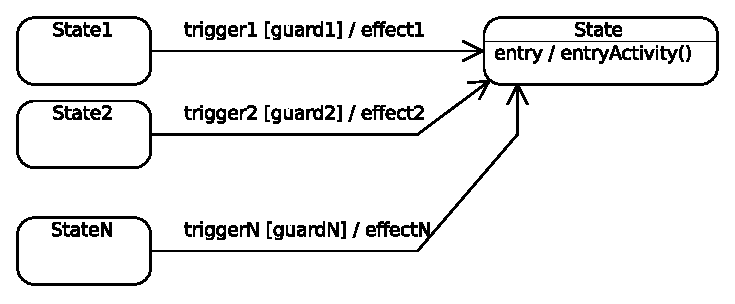
\includegraphics[width=0.7\columnwidth]{images/entryActionsBEFORE}\\ 
(a)\\
  
\includegraphics[width=0.85\columnwidth]{images/entryActionsAFTER}\\
(b)
  \end{tabular}
  \caption{Transformation performed for a {\em State} with an {\tt entry}
activity.}
  \label{fig:entryActions}
\end{figure}

Let us firstly consider a {\em State} having an {\tt entry} activity, as
shown in Figure~\ref{fig:entryActions}(a). Assume that there are $N$ states
({\em State1}, {\em State2}, \ldots, {\em StateN}) that lead to {\em State} when
some guard is fulfilled and triggered, having also associated some effect. The
transformation is performed as follow: for each incoming transition to {\em
State}, a new state is added. This new state is the destination of the incoming
transition, leaving the transition signature (i.e., its trigger, guard and
effect information) as in the original model. Finally, an output transition is
added to the new state that leads to {\em State}. This output transition has no
guard nor trigger event but an effect that correspond to the {\tt entry}
activity of {\em State} before the transformation.
Figure~\ref{fig:entryActions}(b) depicts the transformation performed in a
 model where a {\em State} has an {\tt entry} activity
(Figure~\ref{fig:entryActions}(a)).


\begin{figure}
\centering
  \begin{tabular}{c}
  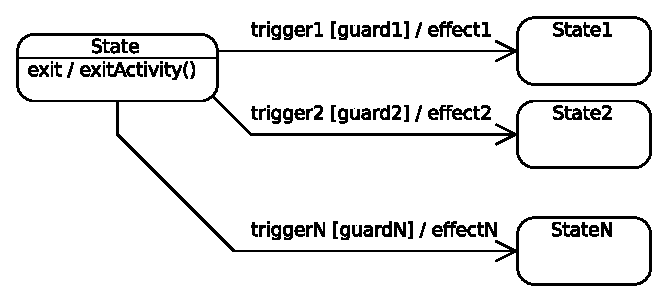
\includegraphics[width=0.7\columnwidth]{images/exitActionsBEFORE}\\ 
(a)\\
  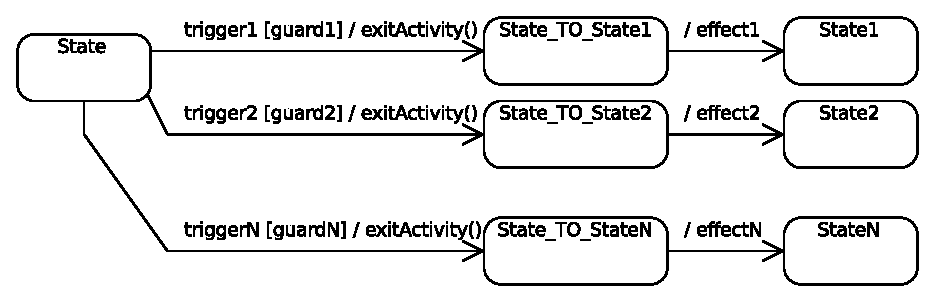
\includegraphics[width=0.85\columnwidth]{images/exitActionsAFTER}\\
(b)
  \end{tabular}
  \caption{Transformation performed for a {\em State} with an {\tt exit}
activity.}
  \label{fig:exitActions}
\end{figure}

Let us consider now a {\em State} having an {\tt exit} activity, as
shown in Figure~\ref{fig:exitActions}(a). Assume that a {\em State} with an
{\tt exit} activity has $N$ different output transitions, each one leading to
different states and being triggered by different event, having a guard and an
effect activity in the transition. In this case, the transformation is
performed as follows: for each output transition of {\em State}, a new states
is added. This new state is the destination of the output transition having as
signature the trigger and the guard of the original model, but changing the
effect to the {\tt exit} activity. Finally, an output transition is added to
the new state leading to the outputs state of the original model. This output
transition has no guard nor trigger event but an effect that correspond to the
effect that was performed when transiting to each state from {\em State} in the
original model. Figure~\ref{fig:exitActions}(b) depicts the transformation
performed in a  model where a {\em State} has an {\tt exit} activity
(Figure~\ref{fig:exitActions}(a)).


\begin{figure}
  \centering
  \begin{tabular}{c}
  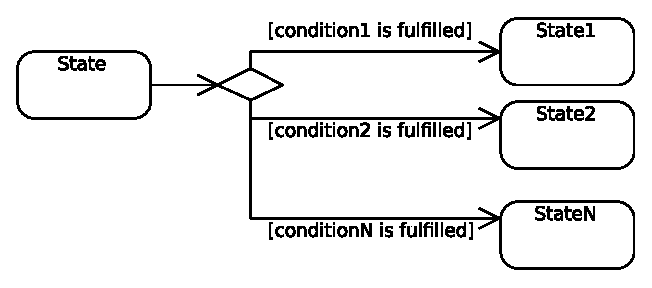
\includegraphics[width=0.7\columnwidth]{images/choiceBEFORE}\\ 
(a)\\
  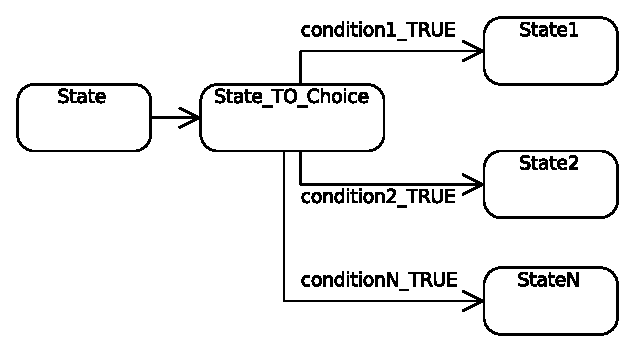
\includegraphics[width=0.7\columnwidth]{images/choiceAFTER}\\
(b)
  \end{tabular}
  \caption{Transformation performed for a {\em State} with a {\tt choice} 
pseudo-state.}
  \label{fig:choicePseudostate}
\end{figure}

Another UML-SM element that we consider in this paper is the {\tt choice}
pseudo-state. A {\tt choice} pseudo-state realises a dynamic conditional
branch, evaluating the guards of the triggers of its outgoing transitions to
select only one outgoing transition. In the case of having more than one
outgoing transitions, any of them can be selected.

Figure~\ref{fig:choicePseudostate}(a) shows a {\em State} having an output {\tt
choice} pseudo-state. Assume that $N$ conditions, when fulfilled, are leading to
a new state. In this case, the transformation is
performed as follows: the {\em choice} pseudo-state is transformed to a state,
having


% Example
\section{Case Study: Train Doors}
\label{sec:casestudy}

This section introduces a case study where we are
interested to verify the model correctness. In this paper, we have considered
a system that models the doors for entering or exiting of a train convoy. Such
a system is  majorly composed by three different elements: a Train Control
Management System (TCMS), a traction system and by several doors. 

The TCMS is an embedded device in charge of supervising the traction system and
the doors. Mainly, it must enable or disable the train traction and the
opening/closing of doors assuring a safe operation of the train.

Figure~\ref{fig:UMLClassDiagram-TrainDoors} depicts the UML Class diagram of
the case study. \TODO{\ldots}



\begin{figure}
  \centering
  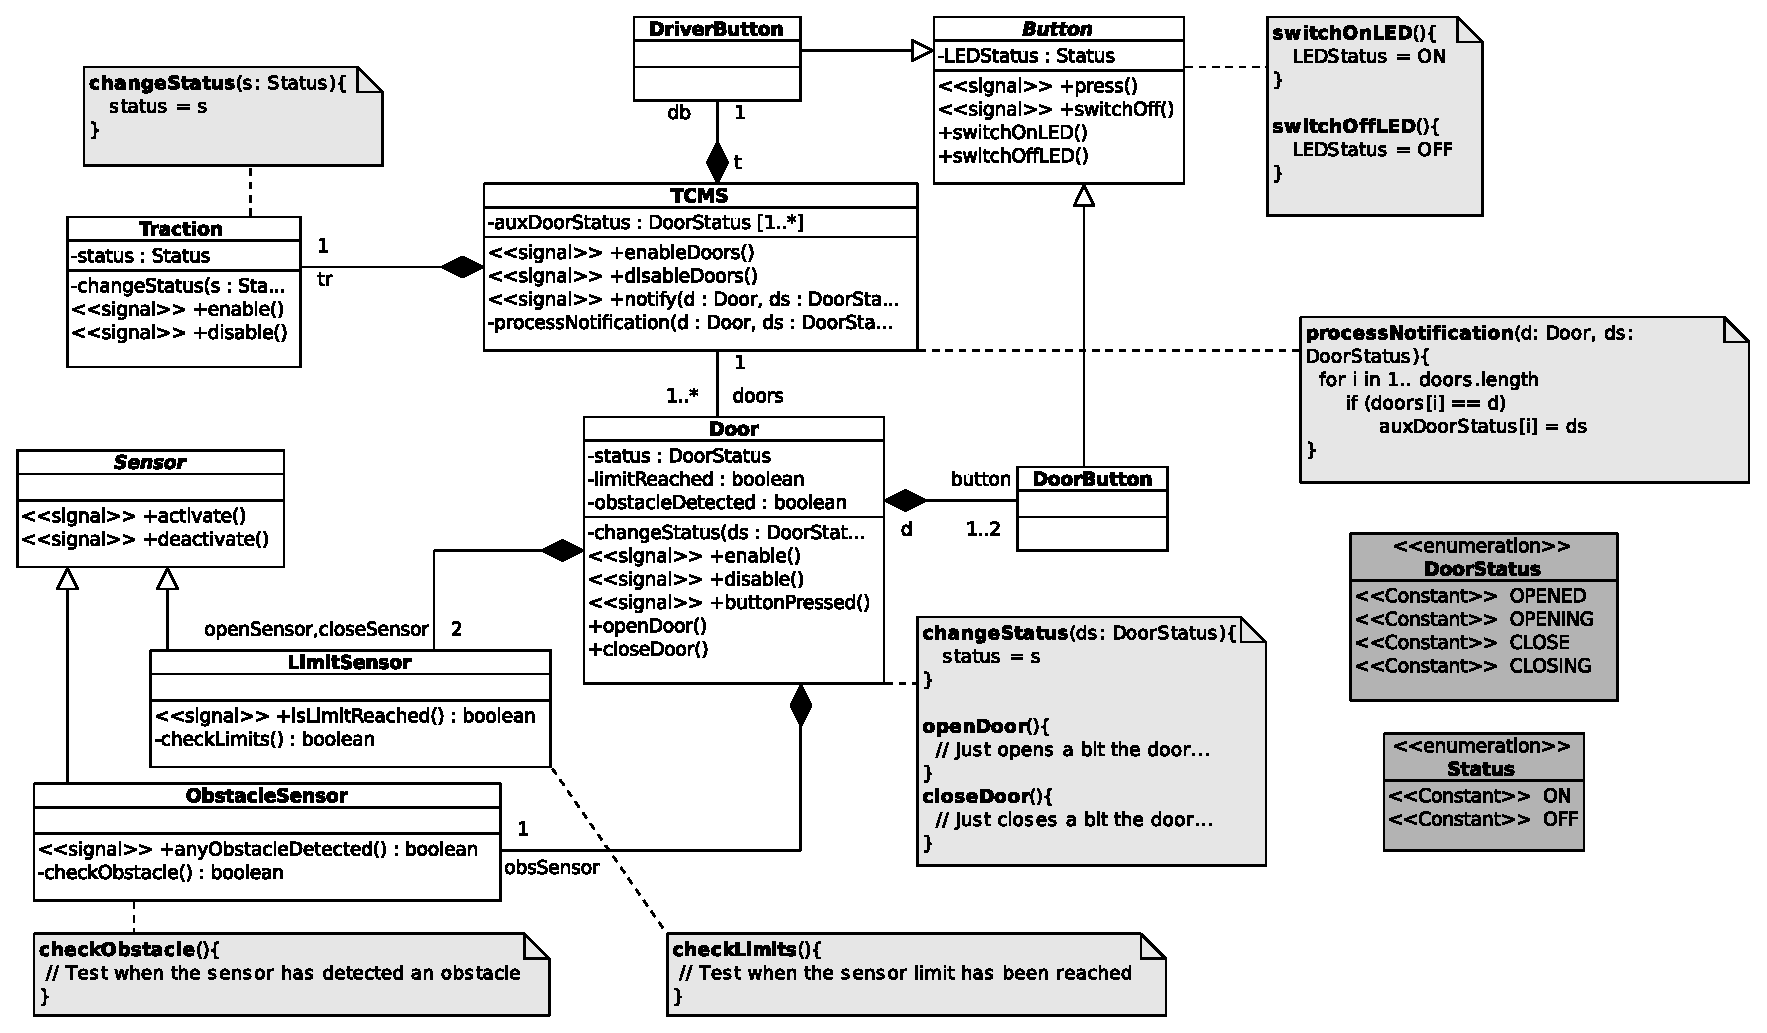
\includegraphics[width=1\columnwidth]{images/UMLClassDiagram-TrainDoors}
  \caption{UML Class diagram for the case study train doors.}
  \label{fig:UMLClassDiagram-TrainDoors}
\end{figure}


\begin{figure}
  \centering
  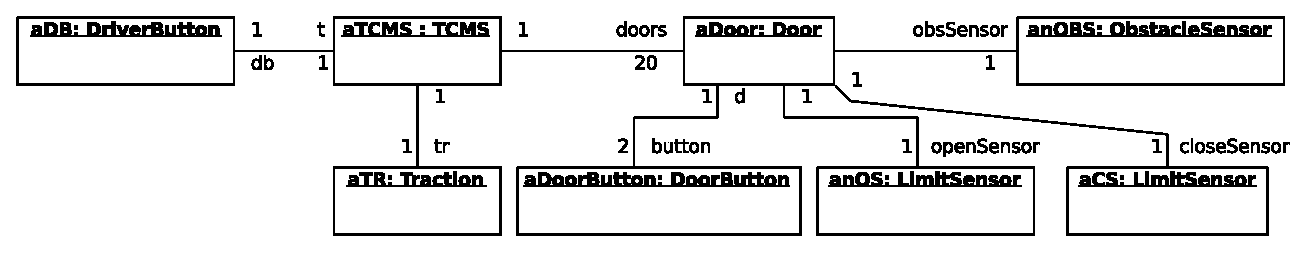
\includegraphics[width=1\columnwidth]{images/UMLObjectDiagram-TrainDoors}
  \caption{.}
  \label{fig:}
\end{figure}


\bibliographystyle{ACM-Reference-Format-Journals}
\bibliography{umerl}

\end{document}

%%% Local Variables: 
%%% mode: latex
%%% TeX-master: t
%%% TeX-PDF-mode: t
%%% ispell-local-dictionary: "british"
%%% End: 
